%%%%%%%%%%%%%%%%%%%%%%%%%%%%%%%%%%%%%%%%%%%%%%%%%%%%%%%%%%%%%%%%%%%%%%%%%%%%%%%
%% PROJECT
%%%%%%%%%%%%%%%%%%%%%%%%%%%%%%%%%%%%%%%%%%%%%%%%%%%%%%%%%%%%%%%%%%%%%%%%%%%%%%%

\section{Project}
\subsection{Research Questions}

\def\rqa{\begin{alertblock}{Research Question 1}
        \rqatext{}
    \end{alertblock}
}

\def\rqb{\begin{alertblock}{Research Question 2}
        \rqbtext{}
    \end{alertblock}
}

\def\rqc{\begin{alertblock}{Research Question 3}
        \rqctext{}
    \end{alertblock}
}

\begin{frame}{Research Questions}
    \rqa{} \vspace*{\fill}
    \rqb{} \vspace*{\fill}
    \rqc{} \vspace*{\fill}
    \vspace{0.2cm}
\end{frame}

\subsection{Methodology}

\begin{frame}{Methodology}
    \framesubtitle{Procedure}
    \rqa{}
    \vspace{0.75cm}
    \begin{enumerate}
        \item \phantomsection{}\label{step:ident-sources}
              Identify authoritative sources on software testing
              %   and ``snowball'' from them
        \item \phantomsection{}\label{step:ident-terms}
              Identify all test approaches and testing-related terms
              %   described in these authoritative sources
        \item \phantomsection{}\label{step:record-info}
              Record data for these terms% all relevant data, including
              %   implicit data, for each term identified in
              %   step~\ref{step:ident-terms}
              ; test approach data are comprised of:
              \vspace*{-0.4cm}\begin{multicols}{3}\begin{enumerate}
                      \item Names
                      \item Categories\footnote{Defined in \Cref{cats-def}.}
                      \item Definitions
                      \item Synonyms\footnote{Defined in \Cref{syn-rels}.}
                      \item Parents\footnote{Defined in \Cref{par-chd-rels}.}
                      \item Flaws\footnote{Defined in \Cref{flaw-def}.}%
                            \phantomsection{}\label{manual-flaws}
                  \end{enumerate}\end{multicols}\vspace*{-0.4cm}
        \item \phantomsection{}\label{step:repeat-process}
              Repeat steps~\ref{step:ident-sources} to \ref{step:record-info} for
              any missing or unclear terms  % until the stopping criteria is reached
              \setcounter{methodCounter}{\value{enumi}}
    \end{enumerate}
    \vspace{1.3cm}
\end{frame}

\begin{frame}{Methodology}
    \framesubtitle{Sources}
    \begin{figure}
        \centering
        \begin{tikzpicture}
            \pie[sum=auto, after number=, text=legend, thick,
                scale=\ifnotpaper0.7\else0.5\fi,
                every label/.style={align=left, scale=0.7}]
            {\stdSources{3}/\stds{},
                \metaSources{3}/\metas{},
                \textSources{3}/\texts{},
                \paperSources{3}/\papers{}}

            \onslide<1>{
                \node[anchor=west, align=center] at (0, 3) {
                    In total, we investigate \srcCount{} sources
                };
            }

            \onslide<2>{
                \node[anchor=west, align=center] at (-2.2, 3) {
                    Textbooks used at McMaster were our ad hoc starting points\\
                    \tiny \citep{Patton2006, PetersAndPedrycz2000, vanVliet2000}
                };
                \draw[->, very thick] (-1.8, 2.9) -- (-1.55, 1.1);
            }

            % \onslide<3>{
            %     \node[anchor=west, align=left] at (2.4, -2) {
            %         Includes websites \citetext{\citealp{LambdaTest2024}; \\
            %             \quad\quad\citealp{Pandey2023}} and a booklet\\
            %         \quad\quad\citep{SPICE2022}};
            %     \draw[->, very thick] (2.25, -1.5) -- (1.25, -1.1);
            % }

        \end{tikzpicture}
    \end{figure}
\end{frame}

\begin{frame}{Methodology}
    \framesubtitle{Terms}
    \begin{itemize}
        \item We build a glossary with a row for each test approach
    \end{itemize}
    \begin{center}
        \begin{table}
            \small
            \begin{tabularx}{\linewidth}{|M{1.1cm}|M{1.3cm}|X|M{1.5cm}|M{1.6cm}|}
                \hline
                \thead{\textbf{Name}} & \thead{\textbf{Category}} & \thead{\textbf{Definition}}                                                                                         & \thead{\textbf{Parent(s)}}                       & \thead{\textbf{Synonym(s)}}           \\
                \hline
                A/B Testing           & Practice {\tiny (Fig.~2)} & Testing ``that allows testers to determine which of two systems or components performs better'' {\tiny (pp.~1, 36)} & Statistical Testing {\tiny (pp.~1,~36)}, \dots{} & Split-Run Testing {\tiny (pp.~1,~36)} \\
                \hline
            \end{tabularx}
            \caption{\tiny Information from \citep{IEEE2022}}
        \end{table}
    \end{center}
    \vspace{-0.5cm}
    \begin{itemize}
        \item We gather this information from sources by looking for:
              \begin{itemize}
                  \item Glossaries, taxonomies, hierarchies, etc.
                  \item Testing-related terms
                  \item Terms described \emph{by} other approaches
                  \item Terms that \emph{imply} other approaches
              \end{itemize}
    \end{itemize}
\end{frame}

% \begin{frame}{Methodology}
%     \framesubtitle{Procedure}
%     \begin{itemize}
%         \item It seems that the existence of a software quality implies the
%               existence of a test type associated with it \pause
%         \item Some test approaches use shared or complicated terminology \pause
%         \item For each of these, we record its
%               \begin{itemize}
%                   \item Name
%                   \item Definition
%                   \item Precedence for a related test type (only for qualities)
%                   \item Synonym(s)
%               \end{itemize}
%     \end{itemize}
% \end{frame}

% \begin{frame}{Methodology}
%     \framesubtitle{Procedure}
%     \begin{itemize}
%         \item Recording these data in a consistent format allows for visualizations to
%               be generated according to a certain logic \pause
%         \item It also allows for subsets of flaws to be identified \pause
%               \vspace{1cm}\rqb{}
%     \end{itemize}
% \end{frame}

\begin{frame}{Methodology}
    \framesubtitle{Procedure}
    \rqb{}
    \begin{enumerate}
        \setcounter{enumi}{\value{methodCounter}}
        \item Automatically analyze recorded test approach data
              \begin{enumerate}
                  \item Visualize approach relations
                  \item Detect certain classes of flaws
                  \item Analyze manually recorded flaws from
                        step~\ref{step:record-info}.\ref{manual-flaws}
              \end{enumerate}
        \item Report results of flaw analysis
              \vspace{0.43cm}
              \rqc{}
        \item Provide examples of how to resolve these flaws
    \end{enumerate}
\end{frame}

\begin{frame}[t]{Methodology}
    \framesubtitle{Categories}
    \vspace{-0.925cm}
    \centering
    \only<1>{\includegraphics[width=\linewidth]{assets/graphs/manual/catRels1.pdf}}
    \only<2>{\includegraphics[width=\linewidth]{assets/graphs/manual/catRels2.pdf}}
    \only<3>{\includegraphics[width=\linewidth]{assets/graphs/manual/catRels3.pdf}}
    \only<4>{\includegraphics[width=\linewidth]{assets/graphs/manual/catRels4.pdf}}
    \only<5>{\includegraphics[width=\linewidth]{assets/graphs/manual/catRels5.pdf}}

    \begin{minipage}{0.98\textwidth}
        % For weird spacing issue
        \only<1-3>{\vspace{-0.8cm}}
        \only<4>{\vspace{-0.475cm}}
        \only<5>{\vspace{0.02cm}}
        \only<1>{\textbf{Approach:} a ``high-level test implementation choice''
            \citep[p.~10]{IEEE2022} used to ``pick the particular test case
            values'' \citeyearpar[p.~465]{IEEE2017}}
        \only<2>{\textbf{Level:} a stage of testing with ``particular
            objectives and \dots{} risks'', each performed in sequence
            (\citealp[p.~12]{IEEE2022}; \citeyear[p.~6]{IEEE2021a};
            \citeyear[p.~6]{IEEE2021c})}
        \only<3>{\textbf{Practice:} a ``conceptual framework that can be applied
            to \dots{} [a] test process to facilitate testing''
            (\citealp[p.~14]{IEEE2022}; \citeyear[p.~471]{IEEE2017})}
        \only<4>{\textbf{Technique:} a
            % ``defined'' and ``systematic'' \citep[p.~464]{IEEE2017}
            ``procedure used to create or select a test
            model, identify test coverage items, and derive corresponding test cases''
            (\citeyear[p.~11]{IEEE2022}; \citeyear[p.~5]{IEEE2021a};
            similar in \citeyear[p.~467]{IEEE2017})}
        \only<5>{\textbf{Type:} ``testing that is focused on specific quality
            characteristics'' (\citealp[p.~15]{IEEE2022}; \citeyear[p.~7]{IEEE2021c};
            \citeyear[p.~473]{IEEE2017})}
    \end{minipage}
\end{frame}

\begin{frame}[t]{Methodology}
    \framesubtitle{Visualization Notation}
    \vspace{-0.925cm}
    \centering
    \only<1>{\includegraphics[width=\linewidth]{assets/graphs/manual/catRels5.pdf}}
    \only<2>{\includegraphics[width=\linewidth]{assets/graphs/manual/catRels6.pdf}}
    \only<3>{\includegraphics[width=\linewidth]{assets/graphs/manual/catRels7.pdf}}

    \begin{minipage}{0.98\textwidth}
        \centering
        % For spacing issues
        \only<1>{\vspace{1.6cm}}
        \only<2>{\vspace{-2.2cm}}
        \only<3>{\vspace{-1.2cm}}
        \only<1>{Arrows point from a \emph{child} node to a \emph{parent} node.}
        \only<2>{Lines without arrowheads connect \emph{synonyms}.}
        \only<3>{Dashed lines indicate a relationship is \emph{implicit}.}
    \end{minipage}
\end{frame}

\begin{frame}[t]{Methodology}
    \framesubtitle{Visualization Notation}
    \begin{columns}[T]
        \begin{column}{.5\textwidth}
            \vspace{-0.5cm}
            \centering
            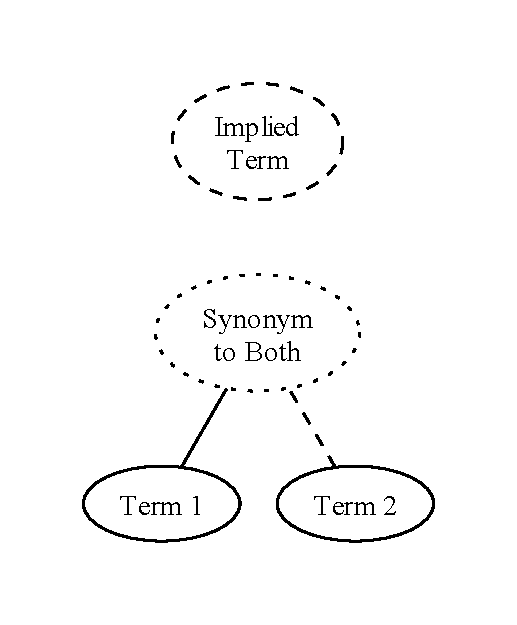
\includegraphics[width=\linewidth]{assets/graphs/manual/catRels8.pdf}
        \end{column}
        \begin{column}{.5\textwidth}
            \vspace{0.75cm}
            Dashed outlines indicate a term is \emph{implicit}.\\
            \vspace{1.3cm}
            Dotted outlines indicate a term is a \emph{synonym} to more than one term.
        \end{column}
    \end{columns}
\end{frame}

\begin{frame}{Visualization of Test Approaches}
    \pause \large \centering \texttt{! Dimension too large.}
    % \includegraphics[width=0.75\textwidth]{assets/graphs/approachGraph.pdf}
\end{frame}

\begin{frame}{Visualization of Test Levels}
    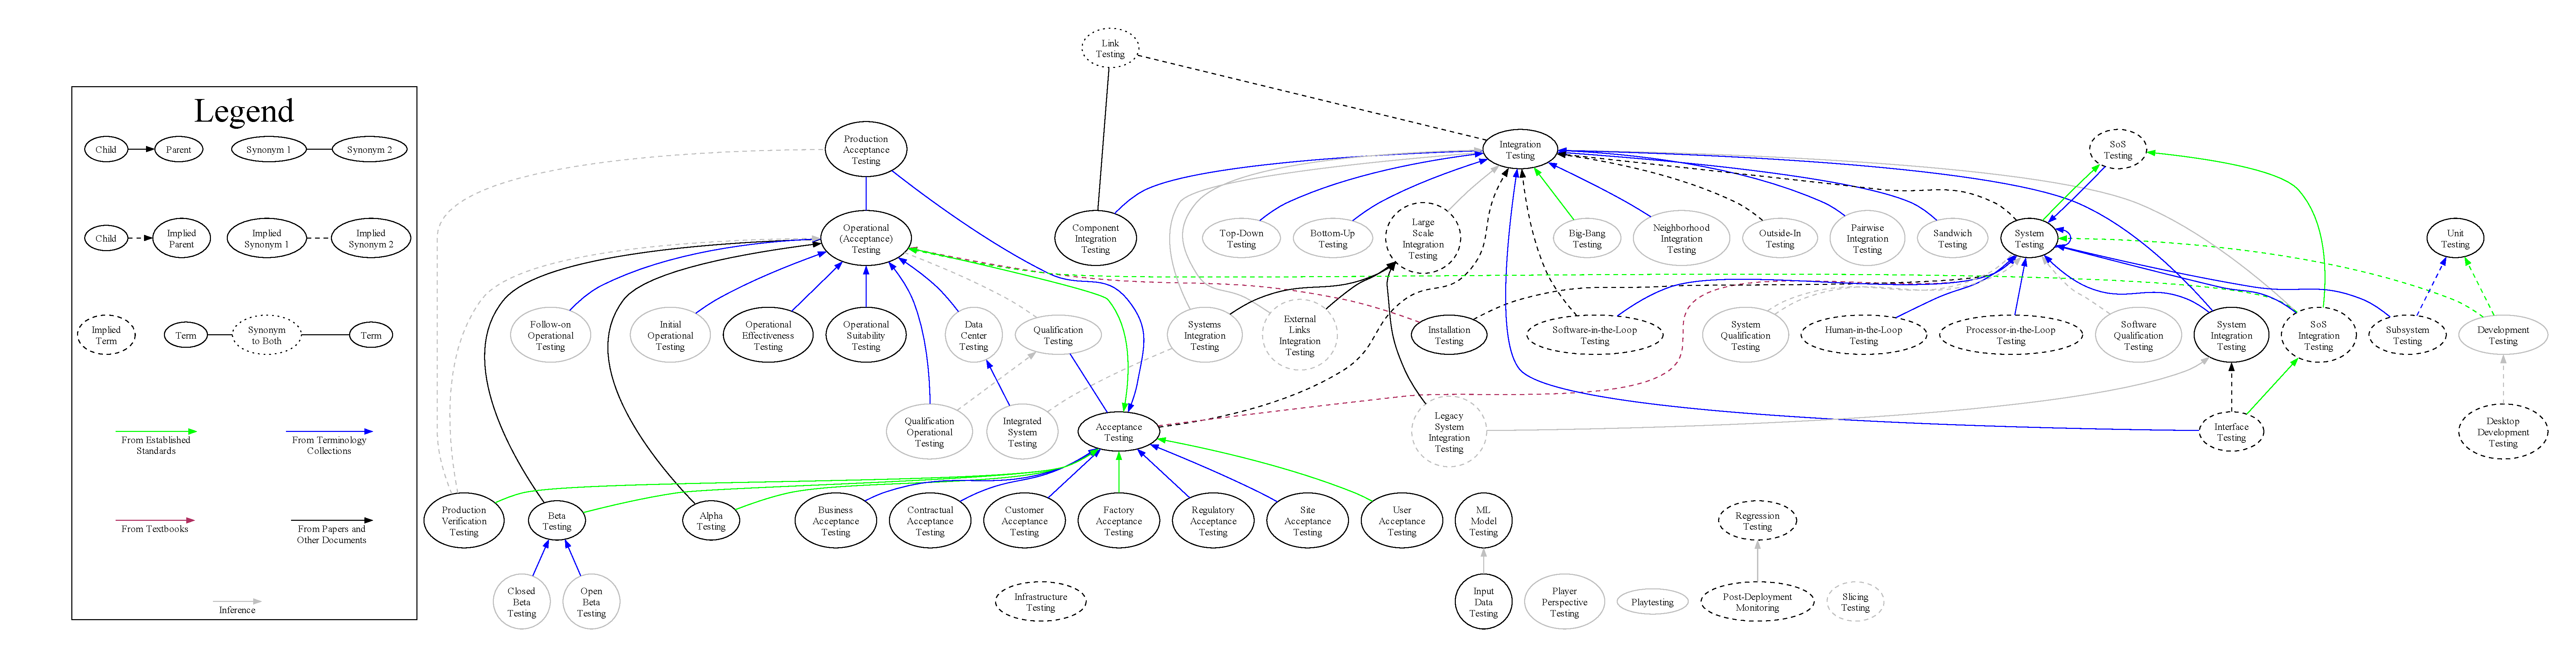
\includegraphics[width=\textwidth]{assets/graphs/levelGraph.pdf}
\end{frame}

\begin{frame}{Visualization of Test Practices}
    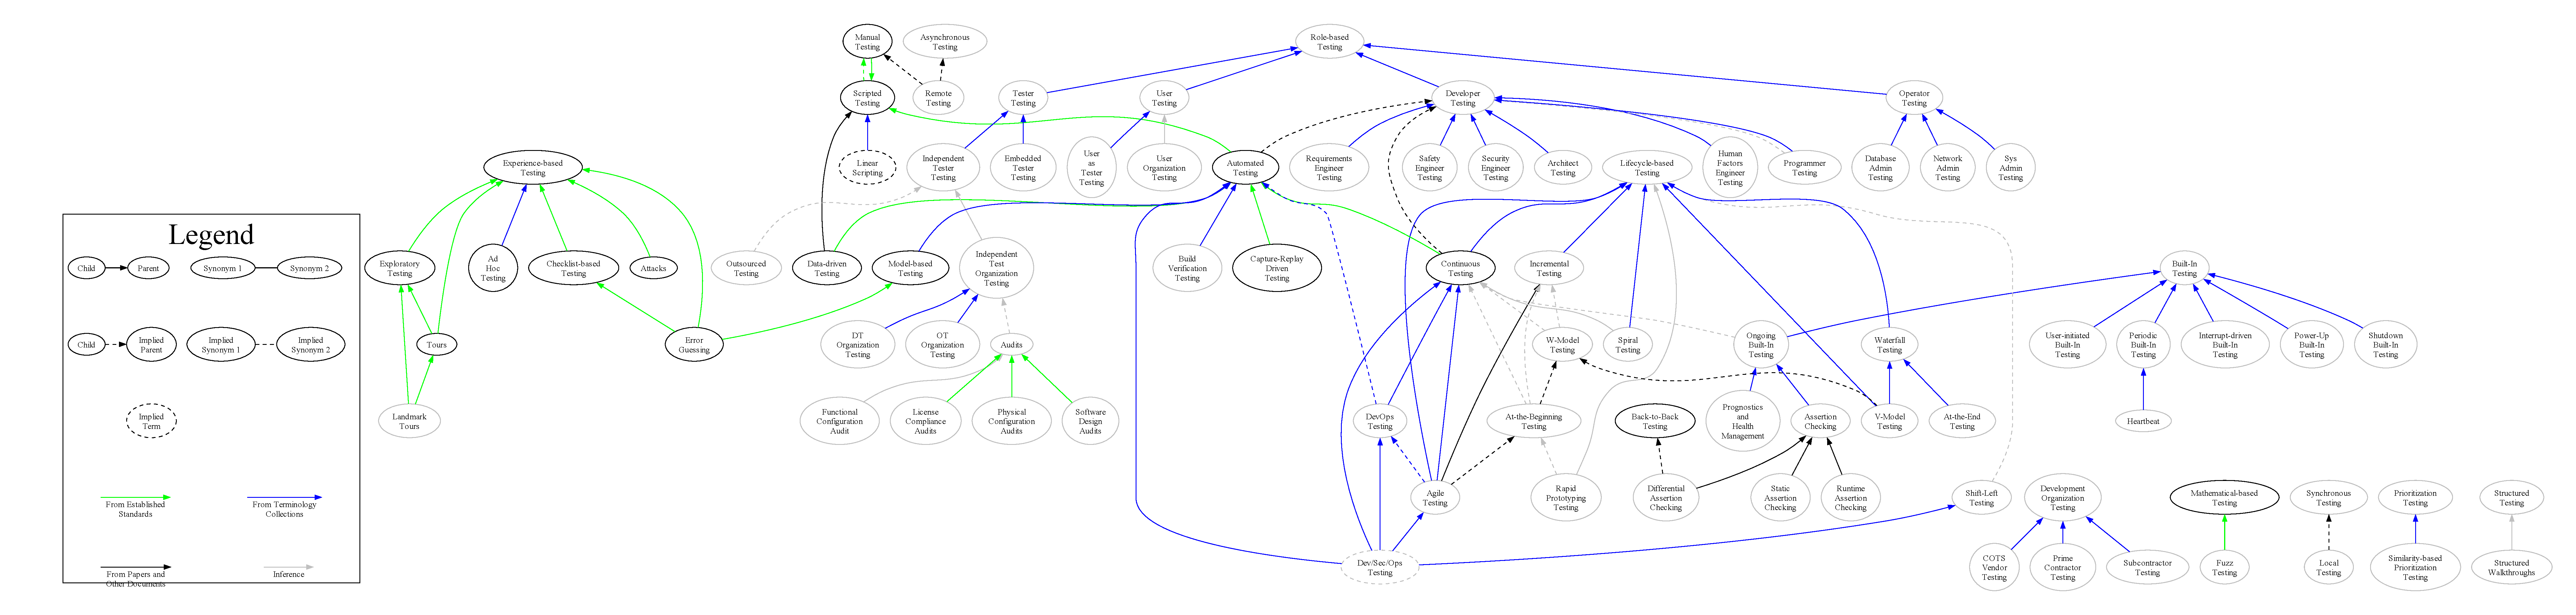
\includegraphics[width=\textwidth]{assets/graphs/practiceGraph.pdf}
\end{frame}

\begin{frame}{Visualization of Test Techniques}
    \includegraphics[width=\textwidth]{assets/graphs/techniqueGraph.pdf}
\end{frame}

\begin{frame}{Visualization of Test Types}
    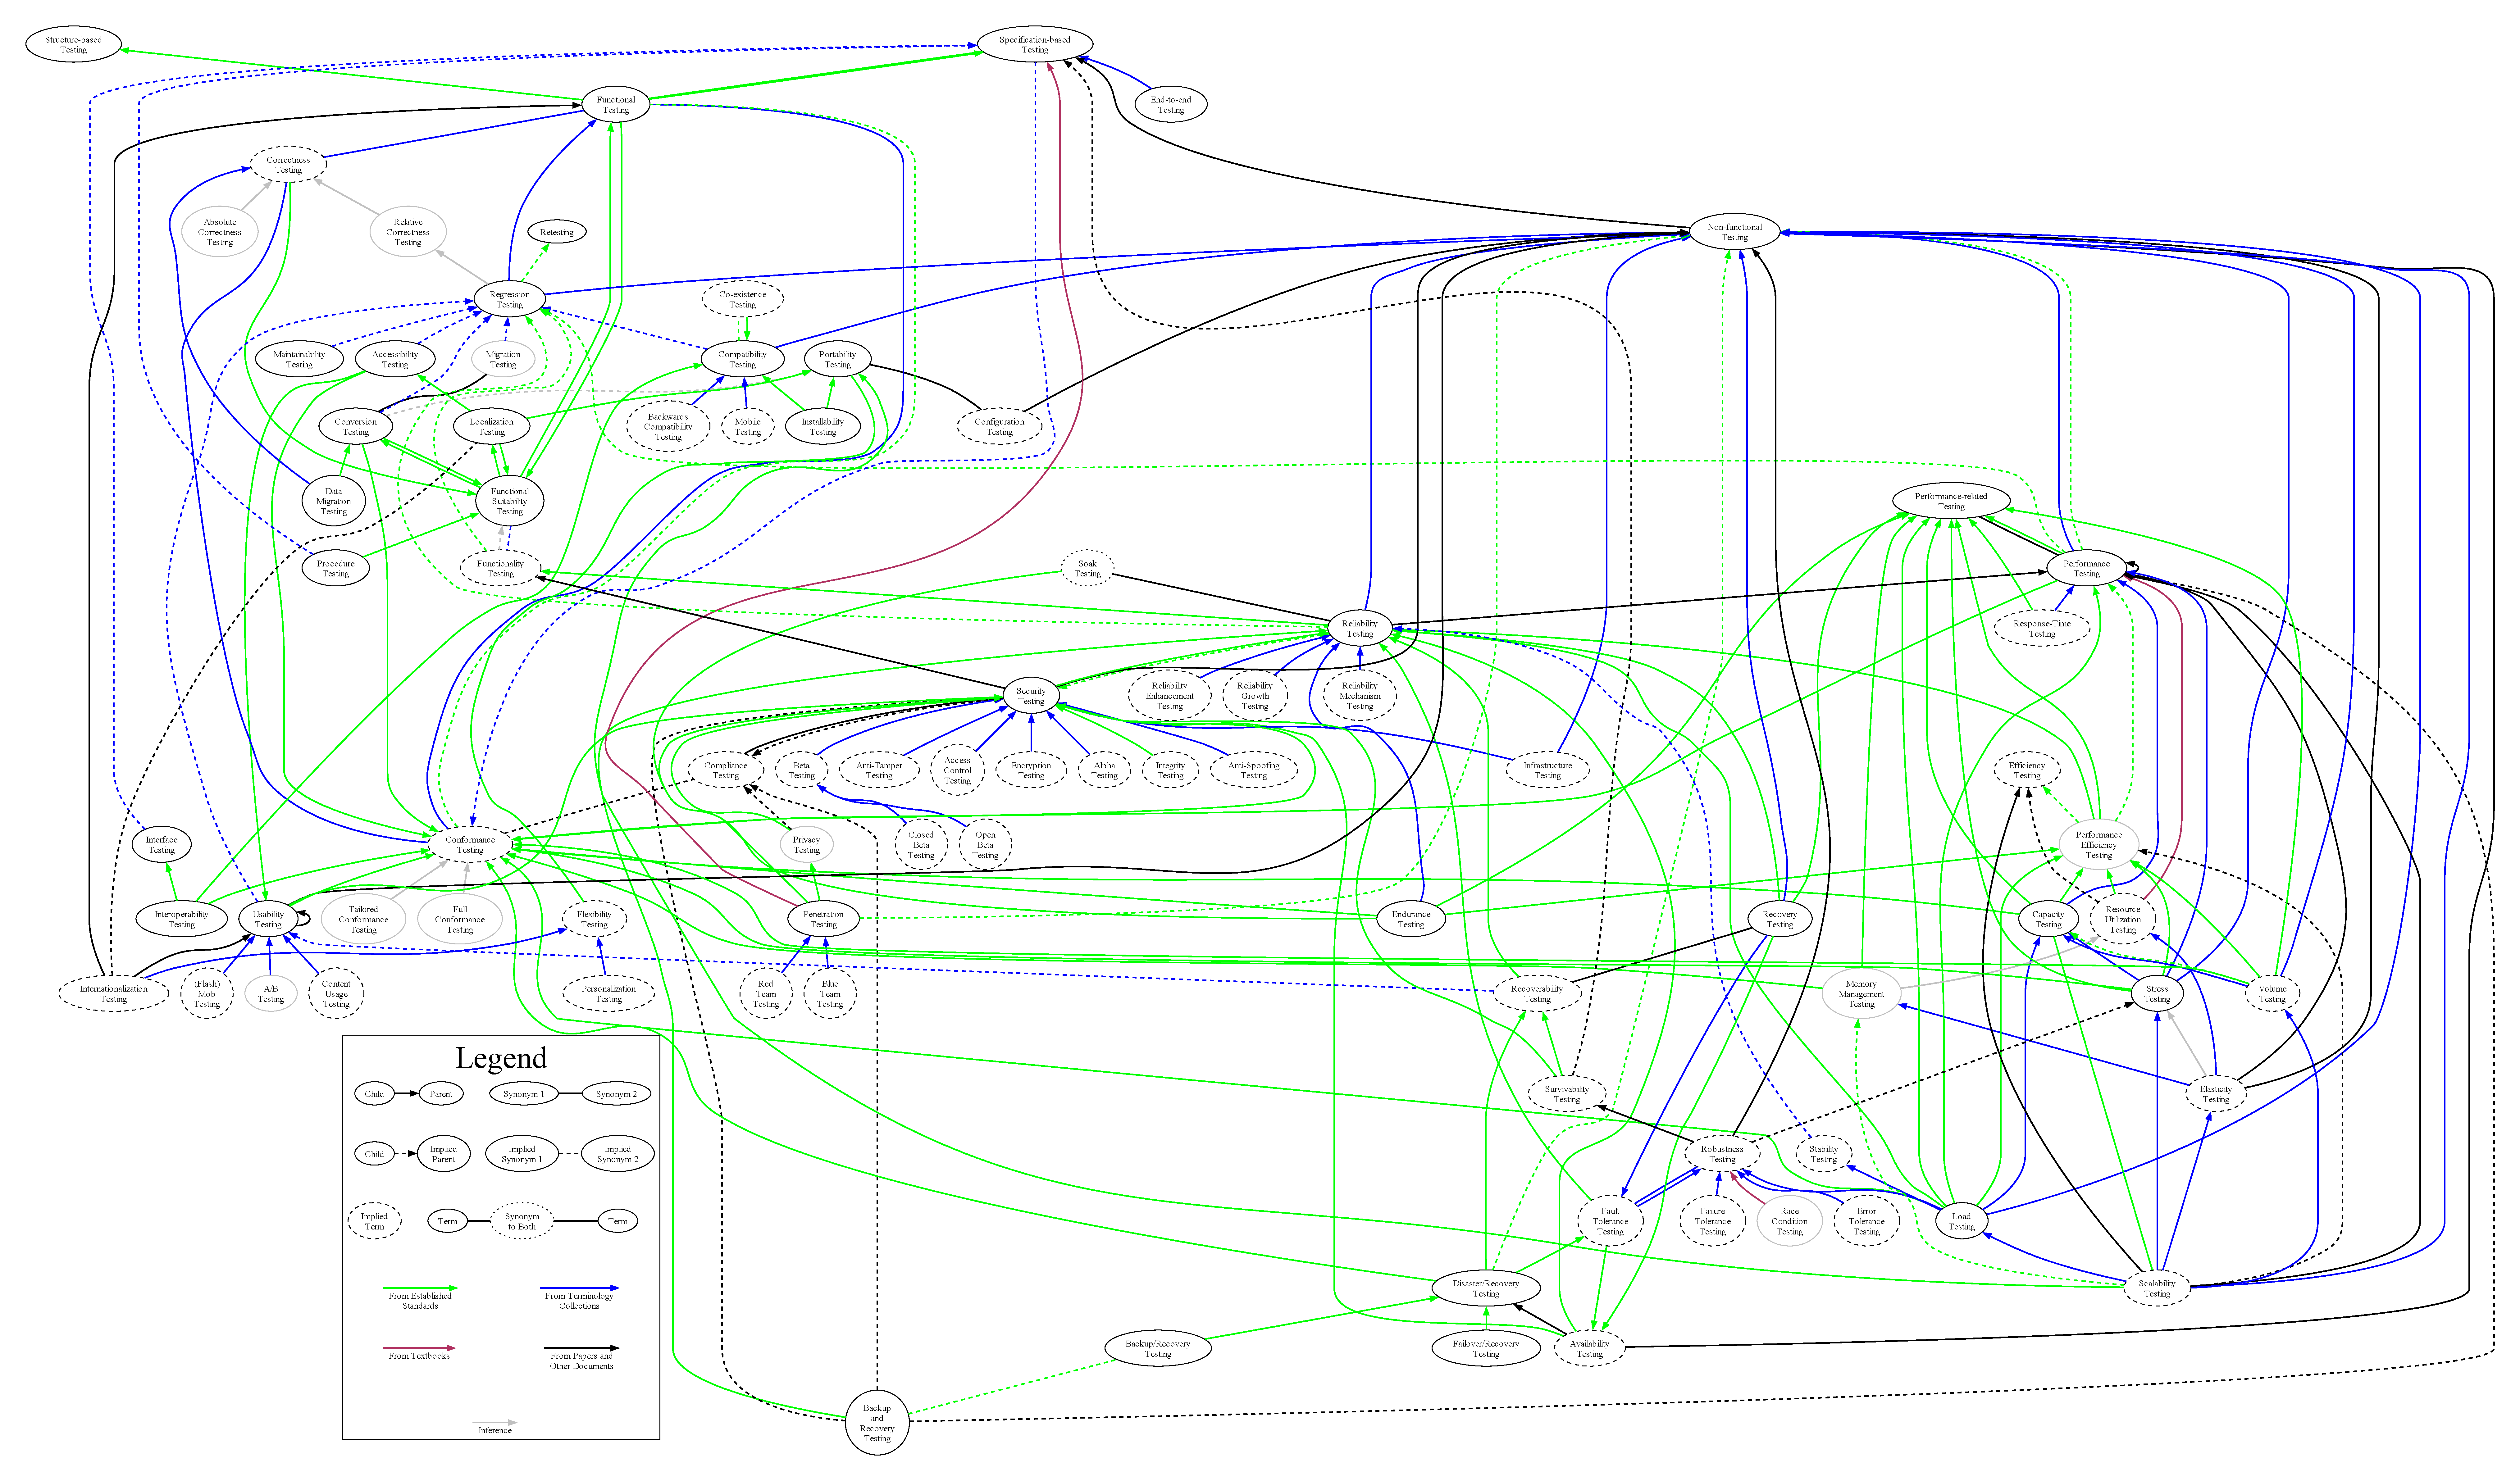
\includegraphics[width=\textwidth]{assets/graphs/typeGraph.pdf}
\end{frame}

% \begin{frame}[t]{Methodology}
%     \framesubtitle{Static Testing}
%     \begin{figure}
%         \centering
%         \includegraphics[height=0.65\textheight]{assets/images/test approach choices}
%         \caption{\tiny \citep[Fig.~2]{IEEE2022}}
%     \end{figure}
% \end{frame}

% \begin{frame}{Methodology}
%     \framesubtitle{Static Testing}
%     \begin{columns}[c]
%         \begin{column}{.3\textwidth}
%             \begin{figure}
%                 \centering
%                 \includegraphics[width=\linewidth]{assets/images/test approach static testing}
%                 \caption{\tiny Adapted from \citep[Fig.~2]{IEEE2022}}
%             \end{figure}
%         \end{column}
%         \begin{column}{.7\textwidth}
%             \begin{itemize}
%                 \item \citeauthor{IEEE2022} seem to describe ``static testing''
%                       as a separate category
%                 \item \pause Is ``static testing'' part of software testing?
%                       \vspace{-0.25cm}\begin{columns}[t]
%                           \begin{column}{.55\textwidth}
%                               \begin{center}
%                                   \textbf{Yes}
%                               \end{center} \tiny
%                               \hspace{0.75cm}\citep[pp.~16\==17]{IEEE2022} \\
%                               \hspace{0.75cm}\citep[p.~43]{IEEE2021b} \\
%                               \hspace{0.75cm}\citep[p.~5\=/2]{SWEBOK2025} \\
%                               \hspace{0.75cm}\citep[pp.~8\==9]{Gerrard2000a}
%                           \end{column}
%                           \begin{column}{.45\textwidth}
%                               \begin{center}
%                                   \hspace{-0.25cm}\textbf{No}
%                               \end{center} \tiny
%                               \citep[p.~427]{IEEE2017} \\
%                               \citep[pp.~5\=/1]{SWEBOK2025} \\
%                               \citep[p.~13]{Firesmith2015} \\
%                               \citep[p.~439]{PetersAndPedrycz2000} \\
%                               \citep[p.~222]{AmmannAndOffutt2017}
%                           \end{column}
%                       \end{columns}\vspace{0.25cm}
%                 \item \pause We record static test approaches for completeness
%                       % \item \pause Quite distinct but not necessarily orthogonal
%                       % \item \pause When considering static testing in isolation,
%                       %       related \emph{dynamic approaches} have grey backgrounds

%                       %       \vspace{-0.5cm}
%                       %       \includegraphics[width=\linewidth]{assets/graphs/manual/catRels9.pdf}
%             \end{itemize}
%         \end{column}
%     \end{columns}
% \end{frame}

% \begin{frame}{Visualization of \emph{Static} Test Approaches}
%     
\includegraphics[width=\textwidth]{assets/graphs/staticGraph.pdf}
% \end{frame}

\section{Results}
\begin{frame}{Overview}
    % \onslide<1->\rqa{} \vspace*{\fill}
    % \onslide<1>\rqb{} \vspace*{\fill}
    % \onslide<1>\rqc{} \vspace*{\fill}
    % \onslide<2>
    % \vspace{-4cm}
    \begin{columns}
        \begin{column}{0.45\textwidth}
            \vspace{-0.5cm}
            \begin{itemize}
                \item \approachCount{} test approaches $\rightarrow$
                \item \qualityCount{} software qualities \\ {\small (may imply test approaches)}
                \item \flawCount{} flaws in the software testing literature
            \end{itemize}
        \end{column}
        \begin{column}{0.55\textwidth}
            \centering
            \begin{tikzpicture}
                \pie[sum=100, text=legend, thick, scale=0.5,
                every label/.style={align=left, scale=0.7}]
                {{\the\numexpr 100 - 100 * \UndefAfter/\TotalAfter}/Defined,
                {\the\numexpr 100 * \UndefAfter/\TotalAfter}/{Not defined}}
            \end{tikzpicture}
        \end{column}
    \end{columns}
\end{frame}

\begin{frame}{Flaw Summary by Source Tier}
    \begin{figure}
        \centering
        \begin{tikzpicture}
\begin{axis}[
width=0.8\textwidth, height=7.5cm,
yticklabels={\parbox{0.24\textwidth}{\raggedleft\papers{}},\parbox{0.24\textwidth}{\raggedleft\texts{}},\parbox{0.24\textwidth}{\raggedleft\metas{}},\parbox{0.24\textwidth}{\raggedleft\stds{}}},
ytick=data,
xlabel=\parbox{0.5\textwidth}{\centering Number of Flaws per Source Tier \\ \quad{}}, xbar, xmin=0,
nodes near coords,
every node near coord/.append style={font=\tiny},
]

\addplot[fill=blue!60] coordinates {(\the\numexpr\paperFlawMnfstBrkdwn{13},0) (\the\numexpr\textFlawMnfstBrkdwn{13},1) (\the\numexpr\metaFlawMnfstBrkdwn{13},2) (\the\numexpr\stdFlawMnfstBrkdwn{13},3)};
\end{axis}
\end{tikzpicture}

\vspace*{0.4mm}
    \end{figure}
\end{frame}

\begin{frame}{Normalized Flaw Summary}
    \begin{figure}
        \centering
        \begin{figure}[bt!]
\centering
\begin{tikzpicture}
\begin{axis}[
width=0.8\textwidth, height=7.5cm,
yticklabels={\parbox{0.24\textwidth}{\raggedleft\papers{}},\parbox{0.24\textwidth}{\raggedleft\texts{}},\parbox{0.24\textwidth}{\raggedleft\metas{}},\parbox{0.24\textwidth}{\raggedleft\stds{}}},
ytick=data,
xlabel=\parbox{0.5\textwidth}{\centering Average Number of Flaws per Document by Source Tier}, xbar, xmin=0,
nodes near coords,
every node near coord/.append style={font=\tiny,/pgf/number format/fixed,/pgf/number format/fixed zerofill,/pgf/number format/precision=1},
]
\pgfmathsetmacro{\stdResult}{\stdFlawMnfstBrkdwn{13} / \stdSources{3}}
\pgfmathsetmacro{\metaResult}{\metaFlawMnfstBrkdwn{13} / \metaSources{3}}
\pgfmathsetmacro{\textResult}{\textFlawMnfstBrkdwn{13} / \textSources{3}}
\pgfmathsetmacro{\paperResult}{\paperFlawMnfstBrkdwn{13} / \paperSources{3}}
\addplot[fill=blue!60] coordinates {(\paperResult,0) (\textResult,1) (\metaResult,2) (\stdResult,3)};
\end{axis}
\end{tikzpicture}

\end{figure}

    \end{figure}
\end{frame}

\begin{frame}{Flaw Summary by Manifestation}
    \begin{center}
        \begin{figure}[bt!]
\centering
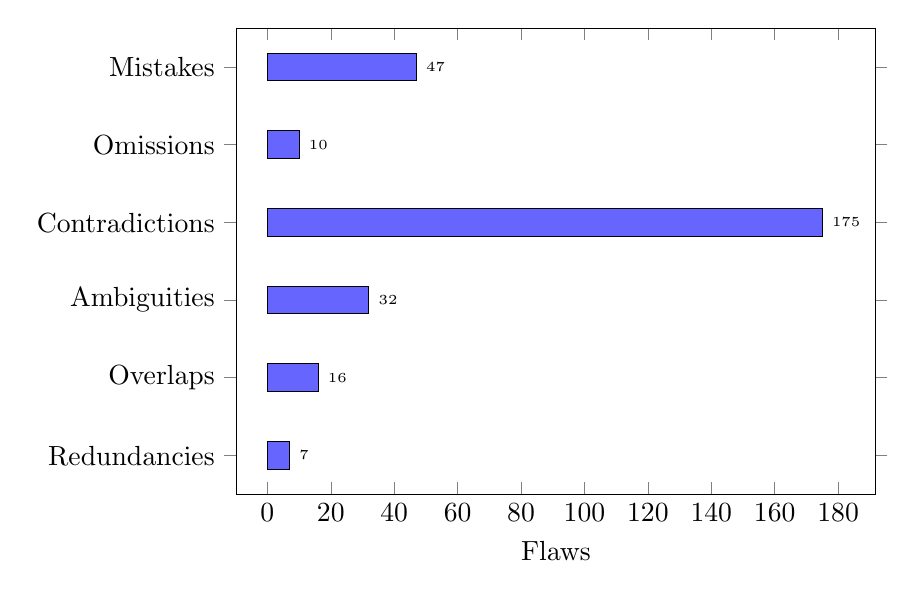
\begin{tikzpicture}
\begin{axis}[
width=0.8\textwidth, height=7.5cm,
symbolic y coords={Redundancies,Overlaps,Ambiguities,Contradictions,Omissions,Mistakes},
ytick=data,
xlabel=Flaws, xbar,
nodes near coords,
every node near coord/.append style={font=\tiny},
]
\addplot[fill=blue!60] coordinates {(7,Redundancies) (16,Overlaps) (32,Ambiguities) (175,Contradictions) (10,Omissions) (47,Mistakes)};
\end{axis}
\end{tikzpicture}
\end{figure}
\hspace{18cm}\vspace*{-8mm}
    \end{center}
\end{frame}

\begin{frame}{Flaw Summary by Domain}
    \begin{center}
        \begin{figure}[bt!]
\centering
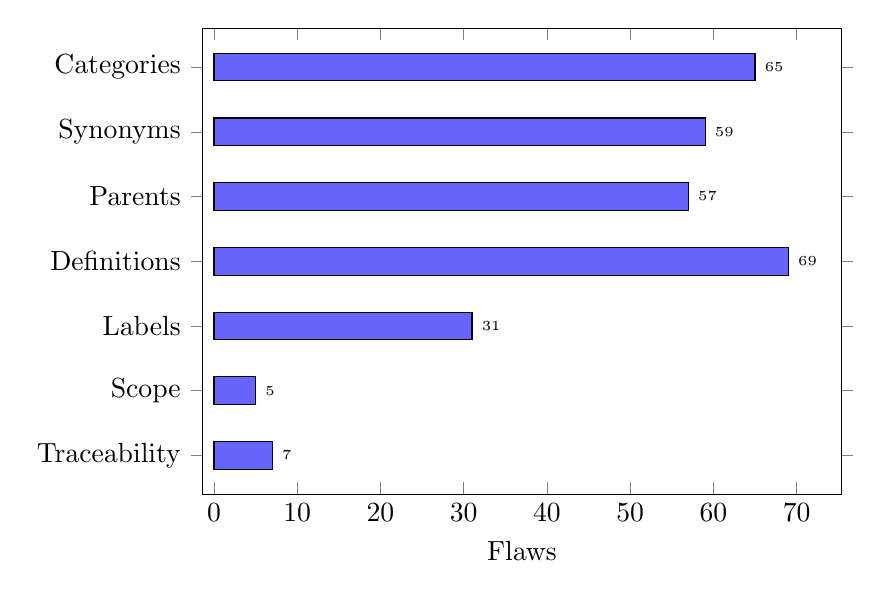
\begin{tikzpicture}
\begin{axis}[
width=0.8\textwidth, height=7.5cm,
symbolic y coords={Traceability,Scope,Labels,Definitions,Parents,Synonyms,Categories},
ytick=data,
xlabel=Flaws, xbar,
nodes near coords,
every node near coord/.append style={font=\tiny},
]
\addplot[fill=blue!60] coordinates {(7,Traceability) (5,Scope) (31,Labels) (69,Definitions) (57,Parents) (59,Synonyms) (65,Categories)};
\end{axis}
\end{tikzpicture}
\end{figure}

    \end{center}
\end{frame}

\begin{frame}{Automated Flaws}
    \framesubtitle{Intransitive Synonyms}
    Some terms are given as a synonym to two (or more) disjoint terms, making
    their relations ambiguous
    \vspace{-0.5cm}
    \begin{columns}[c]
        \begin{column}{.475\linewidth}
            \small
            \begin{table}[hbtp!]
                \centering
                \begin{tabularx}{\textwidth}{c>{\raggedleft\arraybackslash}X} \hline
                    Name & Synonym(s)                                   \\ \hline
                    E    & F (Author, 2022; implied by StdAuthor, 2021) \\
                    G    & F (Author, 2017), H (implied by 2022)        \\
                    H    & X (StdAuthor, 2021)                          \\ \hline
                \end{tabularx}
            \end{table}
        \end{column}
        \begin{column}{.5\linewidth}
            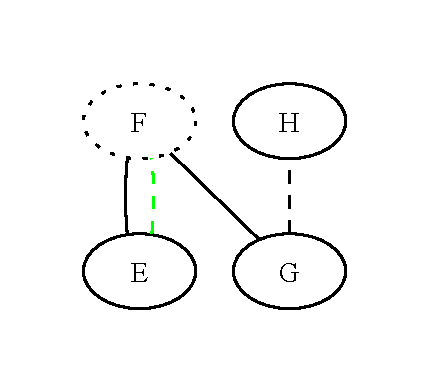
\includegraphics[width=\textwidth]{assets/graphs/SynExampleGlossaryGraph.pdf}
        \end{column}
    \end{columns} %\pause
    \vspace{-0.25cm}
\end{frame}

\begin{frame}{Automated Flaws}
    \framesubtitle{Intransitive Synonyms}
    Some prominent examples: \vspace{0.25cm}
    \begin{enumerate}
        \item \textbf{Functional Testing:} \hfill \textbf{Source(s)}
              \begin{itemize}
                  \item Specification-based Testing {\hfill \tiny \citep[p.~196; \dots{}]{IEEE2017}}
                        %   ; \citealp[pp.~44\==45, 48]{Kam2008}; \citealp[p.~399]{vanVliet2000};
                        % implied by \citealp[p.~129]{IEEE2021c}; \citeyear[p.~431]{IEEE2017})
                  \item \emph{Conformance Testing} {\hfill \tiny \citep[p.~5\=/7]{SWEBOK2025}}
                  \item \emph{Correctness Testing} {\hfill \tiny \citep[p.~5\=/7]{SWEBOK2025}}
              \end{itemize}\pause
              \vspace{0.25cm}
        \item \textbf{Portability Testing:}
              \begin{itemize}
                  \item Flexibility Testing {\hfill \tiny \citep{ISO_IEC2023a}}
                  \item Configuration Testing {\hfill \tiny \citep[p.~43]{Kam2008}}
              \end{itemize}
              \vspace{0.25cm}
        \item \textbf{Soak Testing:}
              \begin{itemize}
                  \item Endurance Testing {\hfill \tiny \citep[p.~39]{IEEE2021c}}
                  \item Reliability Testing {\hfill \tiny (\citealp[Tab.~2]{Gerrard2000a};
                                \citeyear[Tab.~1, p.~26]{Gerrard2000b})}
                        % Endurance testing is given as a child of reliability testing by
                        % \citet[p.~55]{Firesmith2015}, although the terms are not synonyms.
              \end{itemize}
              %   \item \textbf{Link Testing:}
              %   \begin{itemize}
              %       \item Branch Testing {\hfill \tiny (implied by \citealp[p.~24]{IEEE2021c};
              %             \citealp[p.~4]{Reid1996})}
              %       \item Component Integration Testing {\hfill \tiny \citep[p.~45]{Kam2008}}
              %       \item Integration Testing {\hfill \tiny (implied by \citealp[p.~13]{Gerrard2000a})}
              %   \end{itemize}
              % \item \textbf{Invalid Testing:}
              %       \begin{itemize}
              %           \item Error Tolerance Testing {\hfill \tiny \citep[p.~45]{Kam2008}}
              %           \item Negative Testing {\hfill \tiny \citepISTQB{}}
              %       \end{itemize} \pause
    \end{enumerate}
\end{frame}

\begin{frame}{Automated Flaws}
    \framesubtitle{Irreflexive Parents}
    We also find some test approaches that are given as parents of themselves:
    \vspace{0.25cm}
    \begin{enumerate}
        \item Performance Testing {\tiny (\citealp[Tab.~2]{Gerrard2000a}; \citeyear[Tab.~1]{Gerrard2000b})}
        \item System Testing {\tiny \citep[p.~23]{Firesmith2015}}
        \item Usability Testing {\tiny (\citealp[Tab.~2]{Gerrard2000a}; \citeyear[Tab.~1]{Gerrard2000b})}
    \end{enumerate}
\end{frame}

\begin{frame}{Automated Flaws}
    \framesubtitle{Synonym and Parent-Child Overlaps}
    \begin{figure}[h!]
        \centering
        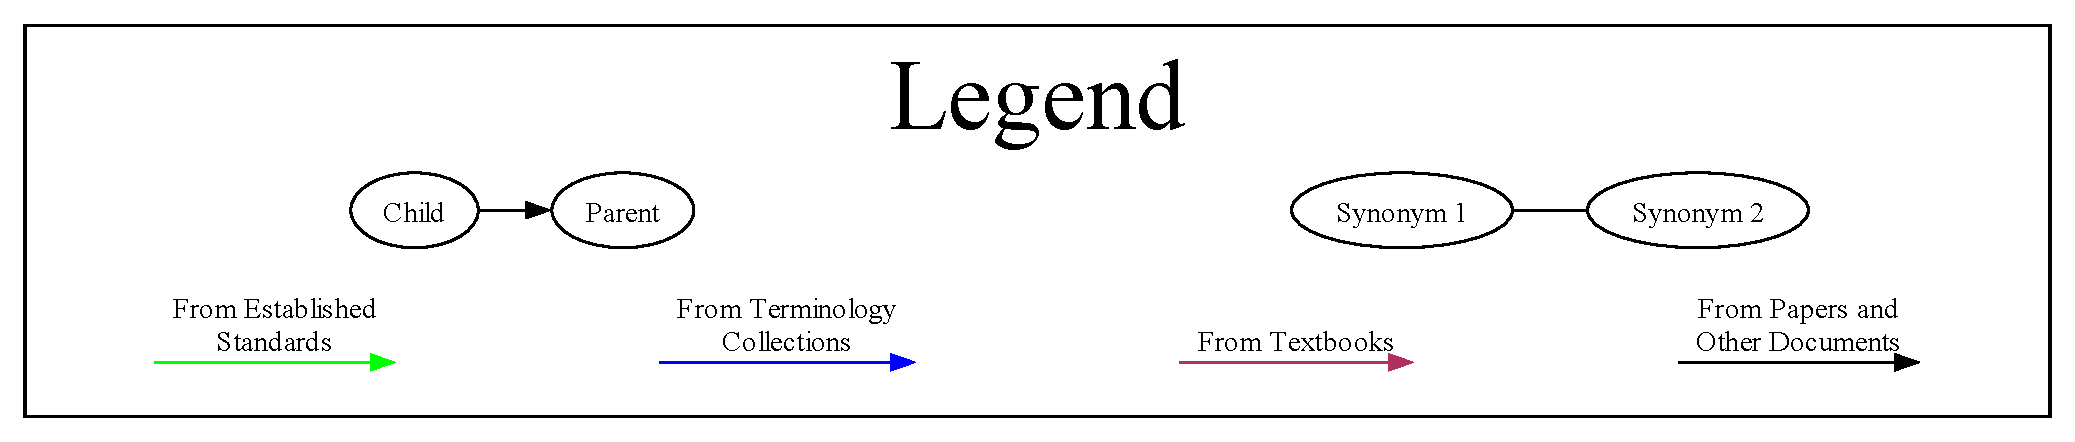
\includegraphics[width=\linewidth]{assets/graphs/manual/expParSynLegend.pdf}
        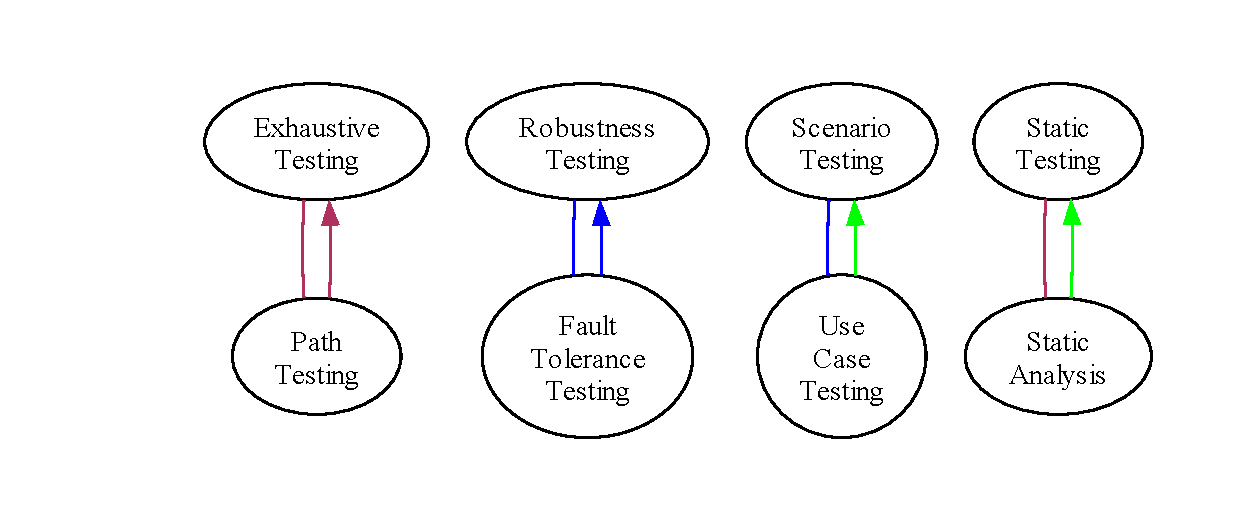
\includegraphics[width=\linewidth]{assets/graphs/manual/expParSynGraph.pdf}
    \end{figure}
\end{frame}

\begin{frame}{Automated Flaws}
    \framesubtitle{Synonym and Parent-Child Overlaps}
    \begin{columns}[c]
        \begin{column}{.4\linewidth}
            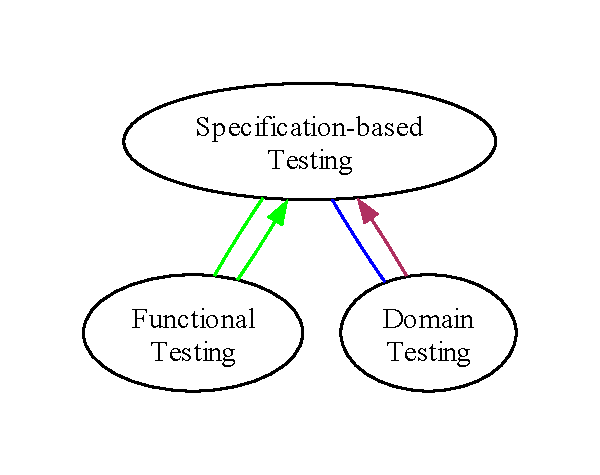
\includegraphics[width=\linewidth]{assets/graphs/manual/expParSynSpecGraph.pdf}
        \end{column}
        \begin{column}{.65\linewidth}
            \begin{itemize}
                \item Functional testing is a:
                      \begin{itemize}
                          \item Synonym {\tiny (\citealp[p.~196]{IEEE2017}; \\\hspace{0.5cm} \citealp[p.~399]{vanVliet2000}; \citealp[pp.~44\==45, 48]{Kam2008}; \dots{})}
                          \item Child {\tiny (\citealp[p.~38]{IEEE2021c}; \citealp[p.~42]{Kam2008})}
                      \end{itemize}
                \item Domain testing is a:
                      \begin{itemize}
                          \item Synonym {\tiny \citep[p.~5\=/10]{SWEBOK2024}}
                          \item Child {\tiny \citep[Tab.~12.1]{PetersAndPedrycz2000}}
                      \end{itemize}
            \end{itemize}
        \end{column}
    \end{columns}
\end{frame}

\begin{frame}{Conclusion}
    \begin{itemize}
        \item The software testing literature is flawed, so
              don't assume everyone is on the same page

              \only<1>{\vspace{0.3cm}
                  \begin{figure}
                      \adjustbox{scale=0.85, center}{
                          \begin{tikzpicture}
\begin{axis}[
width=0.8\textwidth, height=7.5cm,
yticklabels={\parbox{0.24\textwidth}{\raggedleft\papers{}},\parbox{0.24\textwidth}{\raggedleft\texts{}},\parbox{0.24\textwidth}{\raggedleft\metas{}},\parbox{0.24\textwidth}{\raggedleft\stds{}}},
ytick=data,
xlabel=\parbox{0.5\textwidth}{\centering Number of Flaws per Source Tier \\ \quad{}}, xbar, xmin=0,
nodes near coords,
every node near coord/.append style={font=\tiny},
]

\addplot[fill=blue!60] coordinates {(\the\numexpr\paperFlawMnfstBrkdwn{13},0) (\the\numexpr\textFlawMnfstBrkdwn{13},1) (\the\numexpr\metaFlawMnfstBrkdwn{13},2) (\the\numexpr\stdFlawMnfstBrkdwn{13},3)};
\end{axis}
\end{tikzpicture}

}
                  \end{figure}} \pause
        \item Even if they are, there can still be issues!
    \end{itemize}
    \begin{figure}
        \includegraphics[width=0.8\textwidth]{assets/images/system testing}
        \caption{\tiny \citep[p.~23]{Firesmith2015}}
    \end{figure}
\end{frame}
